% Straightness measurement with a Wollaston prism and a straightness reflector
\documentclass[dvisvgm,tikz,border=4pt]{standalone}
% Shared preamble for the TikZ figures in images-1/src (compiled by build.sh)
\usepackage{helvet}
\renewcommand\familydefault{\sfdefault}
\usepackage{amsmath, amssymb}
\usetikzlibrary{arrows.meta, calc, decorations.pathreplacing, patterns, positioning, shapes.geometric, 3d, perspective, fit, backgrounds}
% palette shared with slides.scss and the Graphviz diagrams
\definecolor{dmred}{HTML}{880000}
\definecolor{dmblue}{HTML}{000088}
\definecolor{dmgreen}{HTML}{008800}
\definecolor{dmorange}{HTML}{E08A1E}
\definecolor{ink}{HTML}{333333}
\definecolor{fillblue}{HTML}{E8E8F8}
\definecolor{fillred}{HTML}{F3EAEA}
\definecolor{fillgreen}{HTML}{E8F4E8}
\definecolor{fillorange}{HTML}{FDF0DC}
\definecolor{steel}{HTML}{C9D3DC}
\definecolor{steeldk}{HTML}{8FA3B5}
\definecolor{metal}{HTML}{D9D9D9}
\definecolor{metaldk}{HTML}{A6A6A6}
\tikzset{
  >={Stealth[length=7pt]},
  every picture/.style={line cap=round, line join=round, font=\large},
  proj/.style={gray, dashed, thin},
  dim/.style={<->, >={Stealth[length=5pt]}, thin},
  ext/.style={very thin, gray},
  callout/.style={gray!70!black, thin},
  % datum (origin) symbol
  % pics use absolute sizes so they look the same in mm-scaled drawings
  datum/.pic={
    \fill[white] (0,0) circle (0.22cm);
    \fill[black] (0,0) -- ++(0.22cm,0) arc[start angle=0, end angle=-90, radius=0.22cm] -- cycle;
    \fill[black] (0,0) -- ++(-0.22cm,0) arc[start angle=180, end angle=90, radius=0.22cm] -- cycle;
    \draw[thick] (0,0) circle (0.22cm);
  },
  % reference symbols (absolute sizes): origins have a double circle with a filled quadrant
  wporigin/.pic={
    \draw[thick, fill=white] (0,0) circle (0.3cm);
    \fill[black] (0,0) -- (0.18cm,0) arc[start angle=0, end angle=-90, radius=0.18cm] -- cycle;
    \draw[thick] (0,0) circle (0.18cm);
    \draw (-0.3cm,0) -- (0.3cm,0) (0,-0.3cm) -- (0,0.3cm);
  },
  machorigin/.pic={
    \draw[thick, fill=white] (0,0) circle (0.3cm);
    \fill[black] (0,0) -- (-0.18cm,0) arc[start angle=180, end angle=90, radius=0.18cm] -- cycle;
    \draw[thick] (0,0) circle (0.18cm);
    \draw (-0.3cm,0) -- (0.3cm,0) (0,-0.3cm) -- (0,0.3cm);
  },
  supportpt/.pic={
    \draw[thick, fill=white] (0,0) circle (0.15cm);
    \draw (-0.15cm,0) -- (0.15cm,0) (0,-0.15cm) -- (0,0.15cm);
  },
  regpt/.pic={
    \draw[thick, fill=white] (0,0) circle (0.24cm);
    \draw[thick] (0,0) circle (0.15cm);
    \draw (-0.15cm,0) -- (0.15cm,0) (0,-0.15cm) -- (0,0.15cm);
  },
  % support / registration point (generic)
  target/.pic={
    \draw[thick, fill=white] (0,0) circle (0.12cm);
    \draw (-0.2cm,0) -- (0.2cm,0) (0,-0.2cm) -- (0,0.2cm);
  },
}

\begin{document}
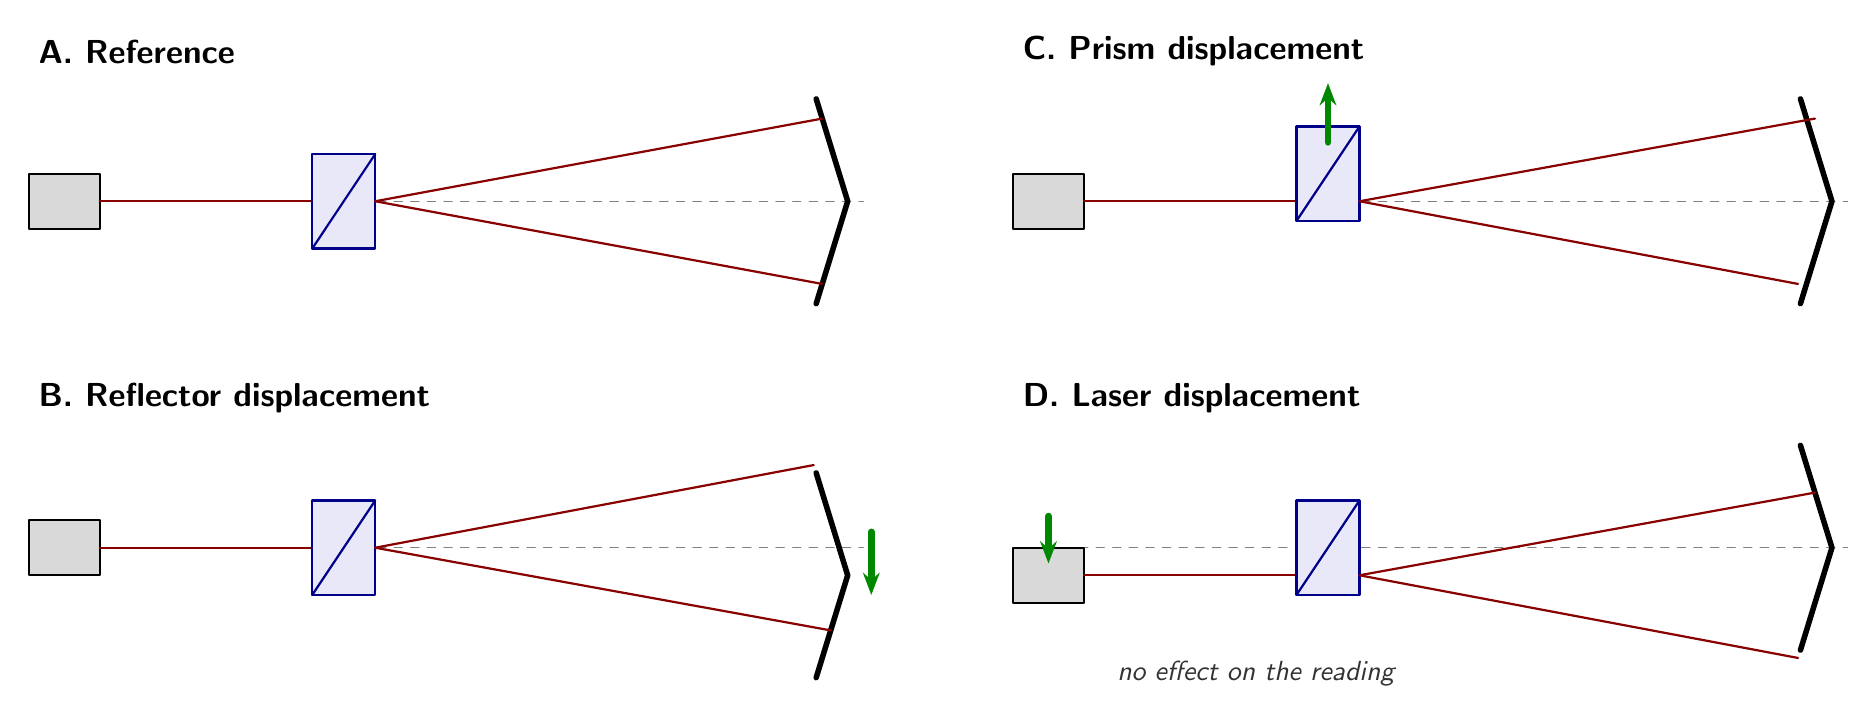
\begin{tikzpicture}[font=\large]
  \tikzset{ray/.style={dmred, thick}, mv/.style={-{Stealth[length=8pt]}, line width=2.5pt, dmgreen}}
  % one panel: \panel{title}{source dy}{prism dy}{mirror dy}
  \newcommand\panel[4]{%
    \node[anchor=west, font=\large\bfseries] at (0,1.9) {#1};
    \draw[dashed, gray] (0,0) -- (10.6,0);
    % laser source
    \draw[thick, fill=metal] (0,#2-0.35) rectangle (0.9,#2+0.35);
    \draw[ray] (0.9,#2) -- (3.6,#2);
    % Wollaston prism: splits the beam into two diverging beams
    \begin{scope}[yshift=#3 cm]
      \draw[thick, fill=fillblue, draw=dmblue] (3.6,-0.6) rectangle (4.4,0.6);
      \draw[thick, dmblue] (3.6,-0.6) -- (4.4,0.6);
    \end{scope}
    % straightness reflector (two mirrors at a small angle), at x = 10
    \begin{scope}[yshift=#4 cm]
      \draw[line width=2pt] (10,-1.3) -- (10.4,0) -- (10,1.3);
    \end{scope}
    \draw[ray] (4.4,#2) -- ({10+0.4*(1-abs(1.05+#2-#3-#4)/1.3)},{1.05+#2-#3+#3});
    \draw[ray] (4.4,#2) -- ({10+0.4*(1-abs(-1.05+#2-#3-#4)/1.3)},{-1.05+#2-#3+#3});
  }
  \begin{scope}             \panel{A. Reference}{0}{0}{0} \end{scope}
  \begin{scope}[xshift=12.5cm] \panel{C. Prism displacement}{0}{0.35}{0}
    \draw[mv] (4,0.75) -- (4,1.5); \end{scope}
  \begin{scope}[yshift=-4.4cm] \panel{B. Reflector displacement}{0}{0}{-0.35}
    \draw[mv] (10.7,0.2) -- (10.7,-0.6); \end{scope}
  \begin{scope}[shift={(12.5,-4.4)}] \panel{D. Laser displacement}{-0.35}{0}{0}
    \draw[mv] (0.45,0.4) -- (0.45,-0.2);
    \node[anchor=west, font=\normalsize\itshape, gray!40!black] at (1.2,-1.6) {no effect on the reading}; \end{scope}
\end{tikzpicture}
\end{document}
